\section{Styrenhet}

\subsection{Hårdvara}

\begin{figure}[H]
  \centering
 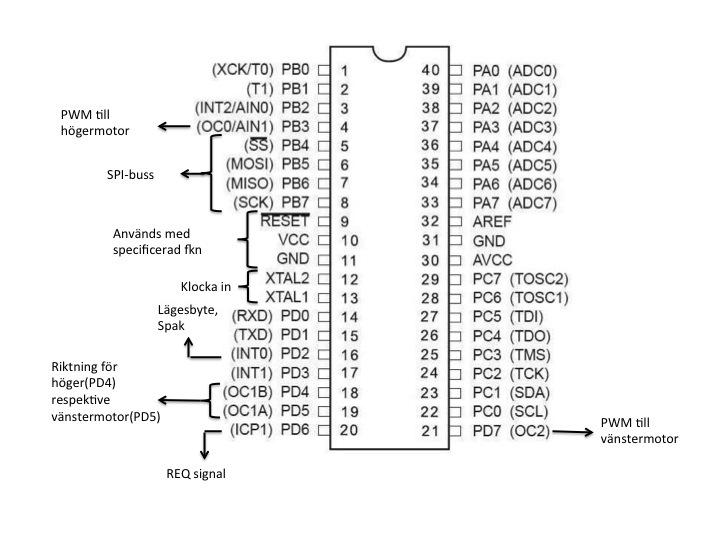
\includegraphics[angle=0,scale=0.5]{bilder/PIN_styr.jpg}
  \caption{Styrenhetens pin-anslutningar}
  \label{fig:PINstyr}
\end{figure}


\subsection{Mjukvara}

\subsubsection{Autonomt läge}

\subsection{Reglering}
Två olika regleralgoritmer används i roboten, en när roboten följer linjer och
en när roboten kör i labyrinter.
\subsubsection{Linjereglering}
TODO: Linjereglering
\subsubsection{Labyrintreglering}
Labyrintregleringen består av 3 olika delar med olika vikter,
en del som ser till att roboten går rakt (P-del), en del som ser till att
roboten håller sig i mitten av labyrinten (M-del) och en del som motverkar
svängningar (D-del).


P-delen använder sig av sidosensorerna för att hålla roboten parallell med
labyrintväggen. En vägg följs i taget, och kommer roboten för nära en vägg så
följs istället den andra väggen. Detta är den huvudsakliga regleringen och har
hög vikt.


M-delen använder sig av frontsensorerna för att hålla sig i mitten av
labyrinten, den försöker att hålla skillnaden mellan höger- och vänstersensorn
till 0. Om det bara finns en vägg att reglera på avaktiveras denna del. Då det
inte är helt avgörande om roboten är i mitten eller lite åt sidan i labyrinten
har denna del låg vikt.


D-delen ser till att roboten rör sig lugnt och inte börjar att oscillera i
labyrinten. Detta gör den genom att kika på skillnaden på sidosensorerna och är
den skillnaden stor så motverkar den P-delen. Eftersom D-delen reglerar på
relativt små skillnader har den hög vikt.

\label{reglering}
